\documentclass[11pt]{article} 
\usepackage[english]{babel}
\usepackage[utf8]{inputenc}
\usepackage[margin=0.5in]{geometry}
\usepackage{amsmath}
\usepackage{amsthm}
\usepackage{amsfonts}
\usepackage{amssymb}
\usepackage[usenames,dvipsnames]{xcolor}
\usepackage{graphicx}
%\usepackage[siunitx]{circuitikz}
\usepackage{tikz}
\usepackage[colorinlistoftodos, color=orange!50]{todonotes}
\usepackage{hyperref}
\usepackage[numbers, square]{natbib}
\usepackage{fancybox}
\usepackage{epsfig}
\usepackage{soul}
\usepackage[framemethod=tikz]{mdframed}
\usepackage[shortlabels]{enumitem}
\usepackage[version=4]{mhchem}
\usepackage{multicol}
\usepackage{forest}
\usepackage{mathtools}
\usepackage{comment}
\usepackage{enumitem}
\usepackage[utf8]{inputenc}
\usepackage[linesnumbered,ruled,vlined]{algorithm2e}
\usepackage{listings}
\usepackage{color}
\usepackage[numbers]{natbib}
\usepackage{subfiles}
%\usepackage{tkz-berge}

\usepackage{listings}
\usepackage{color}
\definecolor{mygreen}{rgb}{0,0.6,0}
\definecolor{mygray}{rgb}{0.5,0.5,0.5}
\definecolor{mymauve}{rgb}{0.58,0,0.82}

\lstset{ 
  backgroundcolor=\color{white},   % choose the background color; you must add \usepackage{color} or \usepackage{xcolor}; should come as last argument
  basicstyle=\footnotesize,        % the size of the fonts that are used for the code
  breakatwhitespace=false,         % sets if automatic breaks should only happen at whitespace
  breaklines=true,                 % sets automatic line breaking
  captionpos=b,                    % sets the caption-position to bottom
  commentstyle=\color{mygreen},    % comment style
  deletekeywords={...},            % if you want to delete keywords from the given language
  escapeinside={\%*}{*)},          % if you want to add LaTeX within your code
  extendedchars=true,              % lets you use non-ASCII characters; for 8-bits encodings only, does not work with UTF-8
  firstnumber=1,                % start line enumeration with line 1
  frame=single,	                   % adds a frame around the code
  keepspaces=true,                 % keeps spaces in text, useful for keeping indentation of code (possibly needs columns=flexible)
  keywordstyle=\color{blue},       % keyword style
  language=Octave,                 % the language of the code
  morekeywords={*,...},            % if you want to add more keywords to the set
  numbers=left,                    % where to put the line-numbers; possible values are (none, left, right)
  numbersep=5pt,                   % how far the line-numbers are from the code
  numberstyle=\tiny\color{mygray}, % the style that is used for the line-numbers
  rulecolor=\color{black},         % if not set, the frame-color may be changed on line-breaks within not-black text (e.g. comments (green here))
  showspaces=false,                % show spaces everywhere adding particular underscores; it overrides 'showstringspaces'
  showstringspaces=false,          % underline spaces within strings only
  showtabs=false,                  % show tabs within strings adding particular underscores
  stepnumber=2,                    % the step between two line-numbers. If it's 1, each line will be numbered
  stringstyle=\color{mymauve},     % string literal style
  tabsize=2,	                   % sets default tabsize to 2 spaces
  title=\lstname                   % show the filename of files included with \lstinputlisting; also try caption instead of title
}

\lstset{
  basicstyle=\ttfamily,
  mathescape
}


\newtheorem{prop}{Proposition}[section]
\newtheorem{thm}{Theorem}[section]
\newtheorem{lemma}{Lemma}[section]
\newtheorem{cor}{Corollary}[prop]

\theoremstyle{definition}
\newtheorem{definition}{Definition}

\theoremstyle{definition}
\newtheorem{required}{Problem}

\theoremstyle{definition}
\newtheorem{ex}{Example}

\setlength{\marginparwidth}{3.4cm}
%#########################################################

%To use symbols for footnotes
\renewcommand*{\thefootnote}{\fnsymbol{footnote}}
%To change footnotes back to numbers uncomment the following line
%\renewcommand*{\thefootnote}{\arabic{footnote}}

% Enable this command to adjust line spacing for inline math equations.
% \everymath{\displaystyle}

% _______ _____ _______ _      ______ 
%|__   __|_   _|__   __| |    |  ____|
%   | |    | |    | |  | |    | |__   
%   | |    | |    | |  | |    |  __|  
%   | |   _| |_   | |  | |____| |____ 
%   |_|  |_____|  |_|  |______|______|
%%%%%%%%%%%%%%%%%%%%%%%%%%%%%%%%%%%%%%%

\title{
\normalfont \normalsize 
\textsc{CSCI 3104 Fall 2021 \\ 
Instructors: Profs. Grochow and Waggoner} \\
[10pt] 
\rule{\linewidth}{0.5pt} \\[6pt] 
\huge Problem Set 1 \\
\rule{\linewidth}{2pt}  \\[10pt]
}
%\author{}
\date{}

\begin{document}

\maketitle


%%%%%%%%%%%%%%%%%%%%%%%%%
%%%%%%%%%%%%%%%%%%%%%%%%%%
%%%%%%%%%%FILL IN YOUR NAME%%%%%%%
%%%%%%%%%%AND STUDENT ID%%%%%%%%
%%%%%%%%%%%%%%%%%%%%%%%%%%
\noindent
Due Date \dotfill September 7, 2021 \\
Name \dotfill \textbf{Didi Trifonova} \\
Student ID \dotfill \textbf{109388776} 
%Collaborators \dotfill \textbf{List Your Collaborators Here}

\tableofcontents

\section{Instructions}
 \begin{itemize}
	\item The solutions \textbf{should be typed}, using proper mathematical notation. We cannot accept hand-written solutions. \href{http://ece.uprm.edu/~caceros/latex/introduction.pdf}{Here's a short intro to \LaTeX.}
	\item You should submit your work through the \textbf{class Canvas page} only. Please submit one PDF file, compiled using this \LaTeX \ template.
	\item You may not need a full page for your solutions; pagebreaks are there to help Gradescope automatically find where each problem is. Even if you do not attempt every problem, please submit this document with no fewer pages than the blank template (or Gradescope has issues with it).

	\item You are welcome and encouraged to collaborate with your classmates, as well as consult outside resources. You must \textbf{cite your sources in this document.} \textbf{Copying from any source is an Honor Code violation. Furthermore, all submissions must be in your own words and reflect your understanding of the material.} If there is any confusion about this policy, it is your responsibility to clarify before the due date. 

	\item Posting to \textbf{any} service including, but not limited to Chegg, Reddit, StackExchange, etc., for help on an assignment is a violation of the Honor Code.

	\item You \textbf{must} virtually sign the Honor Code (see Section \ref{HonorCode}). Failure to do so will result in your assignment not being graded.
\end{itemize}


\section{Honor Code (Make Sure to Virtually Sign)} \label{HonorCode}

\begin{required}
\begin{itemize}
\item My submission is in my own words and reflects my understanding of the material.
\item Any collaborations and external sources have been clearly cited in this document.
\item I have not posted to external services including, but not limited to Chegg, Reddit, StackExchange, etc.
\item I have neither copied nor provided others solutions they can copy.
\end{itemize}

%\noindent In the specified region below, clearly indicate that you have upheld the Honor Code. Then type your name. 
\end{required}

\begin{proof}[I agree to the above - Didi Trifonova]
%% Typing "I agree to the above," followed by your name is sufficient.
\end{proof}


\newpage
\section{Standard 1- Proof by Induction}

\subsection{Problem \ref{Induction1}}
\begin{required} \label{Induction1}
A student is trying to prove by induction that $2^{n} < n!$ for $n \geq 4$. 

\begin{proof}[Student's Proof]
The proof is by induction on $n \geq 4$. 
\begin{itemize}
\item \textbf{Base Case:} When $n = 4$, we have that:
\begin{align*}
2^{4} &= 16 \\
&\leq 24 \\
&= 4!
\end{align*}

\item \textbf{Inductive Hypothesis:} Now suppose that for all $k \geq 4$ we have that $2^{k} < k!$. 

\item \textbf{Inductive Step:} We now consider the $k+1$ case. We have that $2^{k+1} < (k+1)!$. It follows that $2^{k} < k!$. The result follows by induction.
\end{itemize}
\end{proof}

There are two errors in this proof. 
\begin{enumerate}[label=(\alph*)]
\item The Inductive Hypothesis is not correct. Write an explanation to the student explaining why their Inductive Hypothesis is not correct. [\textbf{Note:} You are being asked to explain why the Inductive Hypothesis is wrong, and \textbf{not} to rewrite a corrected Inductive Hypothesis.]


\begin{proof}[Answer]
Instead of ``all $k \geq 4$" it should say ``for some $k \geq 4$" because you are trying to prove that the statement holds true for all $k \geq 4$ . 
\end{proof}



\vskip 15pt
\item The Inductive Step is not correct. Write an explanation to the student explaining why their Inductive Step is not correct. [\textbf{Note:} You are being asked to explain why the Inductive Step is wrong, and \textbf{not} to rewrite a corrected Inductive Step.]

\begin{proof}[Answer]
The inductive step is incorrect because it does not prove that the $k+1$ case is true. This should be accomplished by substituting in the inductive hypothesis somewhere and clearly showing the steps.
\end{proof}
\end{enumerate}
\end{required}





\newpage
\subsection{Problem \ref{Induction2}} 
\begin{required} \label{Induction2}
Consider the recurrence relation, defined as follows:
\[
T_{n} = \begin{cases} 1 & : n = 0, \\
11 & : n = 1, \\
T_{n-1} + 12T_{n-2} & : n \geq 2.
\end{cases}
\]

\noindent Prove by induction that $T_{n} = (-1) \cdot (-3)^{n} + 2 \cdot (4)^{n}$, for all integers $n \in \mathbb{N}$. [\textbf{Recall:} $\mathbb{N} = \{0, 1, 2, \ldots \}$ is the set of non-negative integers.]
\end{required}

\begin{proof}
The proof is by induction on $n \geq 0$. 
\begin{enumerate}
    \item \textbf{Base Cases:} \\
    When n = 0, we have that: 
    \begin{align*}
        T_0 &= (-1)(-3)^0 + 2(4)^0 \\
        &= (-1)(1) + (2)(1) \\
        &= (-1) + 2 = 1 
    \end{align*}
    This proves that for $n = 0$, then $T_0 = 1$ \\
    When n = 1, we have that:
    \begin{align*}
        T_1 &= (-1)(-3)^1 + 2(4)^1 \\
        &= (-1)(-3) + (2)(4) \\
        &= 3 + 8 = 11
    \end{align*}
    This proves that for $n = 1$, then $T_1 = 11$ 
    \item \textbf{Inductive Hypothesis:}
    Assume $T_k = (-1)(-3)^k + 2(4)^k $ is true for some $k \in \mathbb{N}$. 
    \item \textbf{Inductive Step:}
    Prove that $T_{k+1} = (-1)(-3)^{k+1} + 2(4)^{k+1}$ is true. 
    \begin{align*}
            T_{k+1} &= T_k + 12T_{k-1} \\
            &= (-1)(-3)^k + 2(4)^k + 12T_{k-1} \\
            &= (-1)(-3)^k + 2(4)^k + 12[(-1)(-3)^{k-1} + 2(4)^{k-1}]\\
            &= (-1)(-3)^k + 2(4)^k + (-12)(-3)^{k-1} + 24(4)^{k-1} \\
            &= (-1)(-3)^k + 2(4)^k + (-12)(-3)^{-1}(-3)^k + 24(4)^{-1}(4)^k \\
            &= (-1)(-3)^k + 2(4)^k + 4(-3)^k + 6(4)^k \\
            &= [(-1)(-3)^k + 4(-3)^k] + [2(4)^k + 6(4)^k] \\
            &= [(-3)^k(-1+4)] + [(4)^k(2+6)]\\
            &= 3(-3)^k + 8(4)^k \\
            &= (-1)(-3)(-3)^k + 2(4)(4)^k \\
            &= (-1)(-3)^{k+1} + 2(4)^{k+1} 
    \end{align*}
    Therefore, $T_n = (-1)(-3)^n + 2(4)^n$ is true for all $n \in \mathbb{N}$.
\end{enumerate}
\end{proof}

\newpage
\subsection{Problem \ref{Induction3}}
\begin{required} \label{Induction3}
The complete, balanced 4-ary tree of depth $d$, denoted $\mathcal{T}(d)$, is defined as follows. 
\begin{itemize}
\item $\mathcal{T}(0)$ consists of a single vertex.
\item For $d > 0$, $\mathcal{T}(d)$ is obtained by starting with a single vertex and setting each of its four children to be copies of $\mathcal{T}(d-1)$.
\end{itemize}

\noindent Prove by induction that $\mathcal{T}(d)$ has $4^{d}$ leaf nodes. To help clarify the definition of $\mathcal{T}(d)$, illustrations of $\mathcal{T}(0), \mathcal{T}(1)$, and $\mathcal{T}(2)$ are on the next page. [\textbf{Note:} $\mathcal{T}(d)$ is a tree and \textbf{not} the number of leaves on the tree. Avoid writing $\mathcal{T}(d) = 4^{d}$, as these data types are incomparable: a tree is not a number.]
\end{required}

\begin{proof}
The proof is by induction on $d > 0$. \\
**Let $l_d$ be the number of leaf nodes that $T(d)$ has for $d > 0$. \\
\textbf{Theorem 1: With each integer increment of $d$, $l_d$ increases by a factor of 4. } \\
For example: 
\begin{enumerate}
    \item $T(0)$: $l_0 = 1$
    \item $T(1)$: $l_1 = 4$
    \item $T(2)$: $l_2 = 16$
    \item $T(3)$: $l_3 = 64$
    \item $T(4)$: $l_4 = 256$
\end{enumerate}

\begin{enumerate}
    \item \textbf{Base case:} \\
    When d = 0, we have that:
    \begin{align*}
        l_0 &= 4^0 \\
        &= 1
    \end{align*}
    
    \item \textbf{Inductive Hypothesis:} 
    Assume that $l_k = 4^k$ is true for some $k \in \mathbb{N}$. 
    
    \item \textbf{Inductive Step:} 
    Prove that $l_{k+1} = 4^{k+1}$ is true.
    \begin{align*}
        4^{k+1} &= 4^k(4) \\
                &= l_k(4) ^{*} \\
                &= l_{k+1}
    \end{align*}
    * Recall \textbf{theorem 1} where the $T(d+1)$ tree has 4 times as many leaf nodes as the $T(d)$ tree. This is because each previous leaf node creates 4 new leaf nodes when the depth increases by 1. \\ Therefore, $l_d = 4^d$ for all $d \geq 0$.
\end{enumerate}
\end{proof}

\newpage
\begin{ex}
We have the following:

\begin{center}
\begin{forest}
    for tree={
        circle,
        draw,
        fill,
        minimum width=2pt, % size
        inner sep=0pt,
        parent anchor=center,
        child anchor=center,
        s sep+=25pt, % distance between children
    }
[  ]
\end{forest}
\noindent \\ $\mathcal{T}(0)$.
\end{center}

\begin{center}
\begin{forest}
    for tree={
        circle,
        draw,
        fill,
        minimum width=2pt, % size
        inner sep=0pt,
        parent anchor=center,
        child anchor=center,
        s sep+=25pt, % distance between children
    }
[ [] [] []  [] ]
\end{forest}
\noindent \\ $\mathcal{T}(1)$.
\end{center}


\begin{center}
\begin{forest}
    for tree={
        circle,
        draw,
        fill,
        minimum width=2pt, % size
        inner sep=0pt,
        parent anchor=center,
        child anchor=center,
        s sep+=25pt, % distance between children
    }
[ [[] [][] []] [[] [][] []] [[] [][] []] [[] [][] []]  ]
\end{forest}
\noindent \\ $\mathcal{T}(2)$.
\end{center}
\end{ex}

%%%%%%%%%%%%%%%%%%%%%%%%%%%%%%%%%%%%%%%%%%%%%%%%%%


\newpage
\section{Standard 2- BFS and DFS}
\subsection{Problem \ref{DFS1}}
\begin{required} \label{DFS1}
Consider the $\textsf{Connectivity}$ problem:
\begin{itemize}
\item \textsf{Instance:} Let $G(V, E)$ be a simple, undirected graph. Let $u, v \in V(G)$.
\item \textsf{Decision:} Is there a path from $u$ to $v$ in $G$?
\end{itemize}

\noindent \\ Do the following. [\textbf{Note:} There are parts (a) and (b). Part (b) is on the next page.]
\begin{enumerate}[label=(\alph*)]
\item Design an algorithm to solve the $\textsf{Connectivity}$ problem. Your solution should provide enough detail that a CSCI 2270 student could reasonably be expected to implement your solution.
\begin{proof}[Answer for Part (a)] $ $ \\
\textbf{Let $vertices$ be a vector of $vertex$ structs that correspond to $G$} \\
\textbf{Let $adjVertices$ be a vector of all adjacent vertices (data member for $vertex$)} 
\begin{lstlisting}

BFS($vertices$,$u$,$v$)
    for i in 1 to n {
       vertices[i].visited = false % mark each vertex as visited
    }
    q = queue() % create a queue
    q.enqueue(u) % enqueue the source vertex, u 
    while q is not empty{ 
        x = q.front() % assign the front element of q to x
        q.dequeue() % dequeue the front element
        for i in 1 to n { % looping through the adjVertices vector
            % ensure vertices are only visited once 
            if(x -> adjVertices[i].visited == false) 
                if(x -> adjVertices[i] == v) % check for v vertex 
                    return true % return if found
                q.enqueue(x -> adjVertices[i]) % add adjacent to queue
                x -> adjVertices[i].visited = true % mark as visited
        }
        x.visited = true % mark vertex as visited
    }
    return false % will return false if v is not found
\end{lstlisting}
\end{proof}


\newpage
\item We say that the graph $G$ is \textit{connected} if for every pair of vertices $u, v \in V(G)$, there exists a path from $u$ to $v$. Design an algorithm to determine whether $G$ is connected. Your algorithm should only traverse the graph once- this means that you should \textbf{not} apply BFS or DFS more than once. Your solution should provide enough detail that a CSCI 2270 student could reasonably be expected to implement your solution.

\begin{proof}[Answer for Part (b)] $ $ \\
\textbf{Let $vertices$ be a vector of $vertex$ structs that correspond to $G$} \\
\textbf{Let $adjVertices$ be a vector of all adjacent vertices (data member for $vertex$)} 
\begin{lstlisting}
BFS($vertices$,$u$,$v$)
    int numVisited = 0
    for i in 1 to n {
       vertices[i].visited = false % mark each vertex as unvisited
    }
    q = queue() % create a queue
    q.enqueue(u) % enqueue the source vertex, u 
    while q is not empty{ 
        x = q.front() % assign the front element of q to x
        q.dequeue() % dequeue the front element
        for i in 1 to n { % looping through the adjVertices vector
            % ensure vertices are only visited once 
            if(x -> adjVertices[i].visited == false) 
                x -> adjVertices[i].visited = true % mark as visited
                % *Increment every time a new vertex is visited
                numVisited++ 
                q.enqueue(x -> adjVertices[i]) % add adjacent to queue
        }
        if(x.visited == false) 
            numVisited++ % increment once again 
            x.visited = true % mark vertex as visited
    }
    return numVisited
\end{lstlisting}
Once the while loop terminates, compare the $numVisited$ variable with the size of the $vertices$ vector. If $numVisited = vertices.size$, then the graph is connected because every vertex was visited using BFS from the first vertex in the vector. If $numVisited < vertices.size$, then the graph is disconnected because there are one or more vertices that were not visited by starting with the initial vertex.
\end{proof}
\end{enumerate}
\end{required}


\newpage
\subsection{Problem \ref{DFS2}} 
\begin{required} \label{DFS2}
Give an example of a simple, undirected, and unweighted graph $G(V, E)$ that has a single source shortest path tree which a \textbf{depth-first traversal} will not return for any ordering of its vertices. 
    Your answer must
    \begin{enumerate}[label=(\alph*)]
    	\item Provide a drawing of the graph $G$. [\textbf{Note:} We have provided TikZ code below if you wish to use \LaTeX \ to draw the graph. Alternatively, you may hand-draw $G$ and embed it as an image below, provided that (i) your drawing is legible and (ii) we do not have to rotate our screens to grade your work.]
    	\item Specify the single source shortest path tree $T = (V,E_T)$ by specifying $E_T$ and also specifying the root $s \in V$. [\textbf{Note:} You may again hand-draw this tree. If you wish, you may clearly mark the edges of $T$ on your drawing of $G$. Please make it easy on the graders to identify the edges of $T$.] 
    	\item Include a clear explanation of why the depth-first search algorithm we discussed in class will never produce $T$ for any orderings of the vertices.
    \end{enumerate}

\end{required}

\noindent 
\begin{proof}[Answer] $ $ \\
(a) G, where DFS will not produce a SSSP tree \\
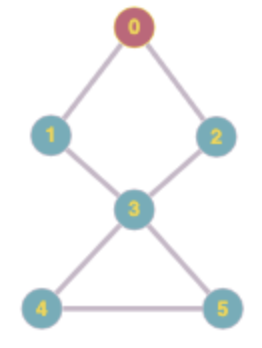
\includegraphics[]{image1.png} \\
(b) $T = (V, E_T)$ (Using BFS) \\
 $E_T = \{(0,1), (0,2), (1,3), (3,4), (3,5)\}$ \\
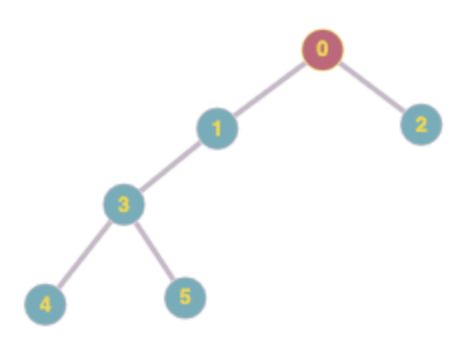
\includegraphics[]{image2.png} \\
(c) Below is an example of the tree produced from part (a) using DFS.\\ 
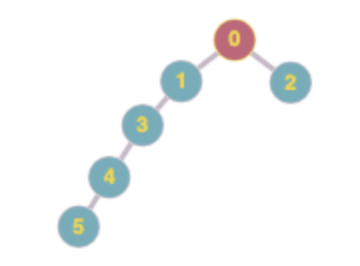
\includegraphics[]{image3.png} \\
This is clearly not a SSSP tree because the path from 0 to 5 is (0,1,3,4,5) when the shortest path in G is actually (0,1,3,5). This is because DFS goes as far down a path as possible instead of first examining the closest depth. By going to the closest depth first (BFS), then you use the least amount of edges before reaching the destination vertex.  
%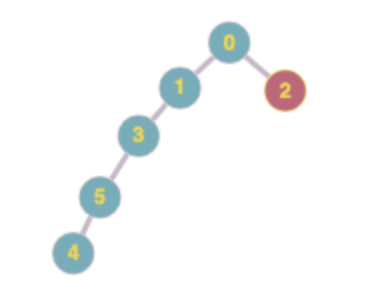
\includegraphics[]{image4.png} 

\end{proof}





\newpage
\subsection{Problem \ref{DFS4}}
\begin{required} \label{DFS4}
	Give an example of a simple, undirected, weighted graph such that a breadth-first traversal outputs a search-tree that is not a single source shortest path tree. (That is, BFS is not sufficiently powerful to solve the shortest-path problem on weighted graphs. This motivates Dijkstra's algorithm, which will be discussed in the near future.) 
	Your answer must
	\begin{enumerate}[label=(\alph*)]
		\item Draw the graph $G = (V,E, w)$ by specifying $V$ and $E$, clearly labeling the edge weights.  [\textbf{Note:} We have provided TikZ code below if you wish to use \LaTeX \ to draw the graph. Alternatively, you may hand-draw $G$ and embed it as an image below, provided that (i) your drawing is legible and (ii) we do not have to rotate our screens to grade your work.]
		\item Specify a spanning tree $T(V, E_{T})$ that is returned by BFS, but is not a single-source shortest path tree. [\textbf{Note:} You may again hand-draw this tree. If you wish, you may clearly mark the edges of $T$ on your drawing of $G$. Please make it easy on the graders to identify the edges of $T$.] 

		\item Specify a valid single-source shortest path tree $T^{\prime} = (V,E_{T^{\prime}})$.  [\textbf{Note:} You may again hand-draw this tree. If you wish, you may clearly mark the edges of $T$ on your drawing of $G$. Please make it easy on the graders to identify the edges of $T$.] 

		\item Include a clear explanation of why the search-tree output by breadth-first search is not a valid single-source shortest path tree of $G$.
	\end{enumerate}
\end{required}


\begin{proof}[Answer] $ $\\
(a) G, where BFS does not produce a SSSP Tree \\
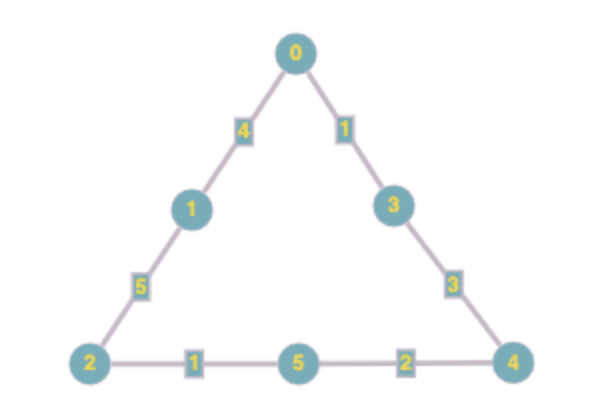
\includegraphics[]{image6.png} \\
(b), a spanning tree that is returned by BFS but not a SSSP tree (on next page).\\
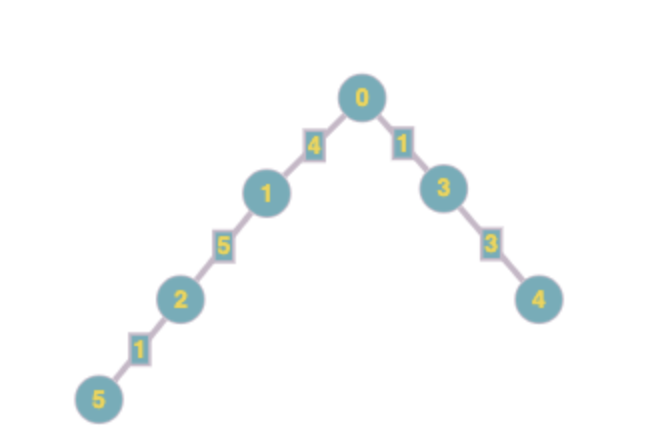
\includegraphics[]{image7.png} \\
(c) Valid SSSP Tree \\
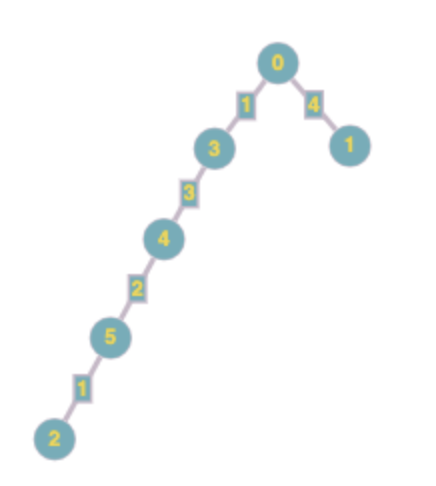
\includegraphics[]{image8.png} \\
(d) BFS is not a valid method of finding the shortest path in this scenario because the edges are weighted. In part b, the path from 0 to 2 yields a total length of 9. However, in part c, the path from 0 to 2 yields a length of 7. Even though it takes 2 times as many edges, the edges are weighted much less and results in a shorter length overall. 
\end{proof}


\end{document} % NOTHING AFTER THIS LINE IS PART OF THE DOCUMENT



